\documentclass[11pt,a4paper]{article}
\usepackage{amsmath,amssymb,graphicx,booktabs,hyperref,siunitx}
\usepackage[margin=2.5cm]{geometry}
\graphicspath{{figures/}}

\title{Quadrature All-Pass Topologies for UHJ\\\large A Multi-Rate Comparative Study}
\author{Giuseppe Silvi --- SEAM}
\date{2026}

\begin{document}
\maketitle
\begin{abstract}
This study compares the all-pass network topologies that realise a wideband 90-degree quadrature for UHJ encoding.
It measures phase accuracy, computational cost, sample-rate behaviour, and group delay on one harness, and it recommends a topology for a standalone quadrature plugin.
\end{abstract}
\tableofcontents

%% ─── §1 Introduction ─────────────────────────────────────────────────────────
\section{Introduction}

The UHJ encoding matrix requires a wideband 90-degree phase shift — the
\emph{j} operator — applied across the full audible spectrum with sub-degree
accuracy.
Two questions organise this study: which all-pass topology delivers the
greatest phase accuracy per unit computational cost, and how each topology
behaves as the sample rate changes from \SI{44.1}{\kilo\hertz} to
\SI{192}{\kilo\hertz}.

The problem has a continuous history.
Analog phase-difference networks, analysed by Bedrosian \cite{Bedrosian1960},
showed that cascaded first- and second-order all-pass sections can approximate
a 90-degree differential phase over a prescribed bandwidth.
Schroeder's 1958 differential all-pass arrangement is the conceptual origin of
transforming a mono signal into a perceived stereo image through phase
manipulation; its design goal was decorrelation rather than a held quadrature
relationship, yet it established the building block that later work would
repurpose.
Gerzon applied the quadrature idea to UHJ surround encoding
\cite{gerzon1983broadcast}, where a precise 90-degree shift converts
mid-side signals into the spatially encoded B-format lateral component.
The modern digital realisation rests on the lattice all-pass section studied by
Regalia, Mitra, and Vaidyanathan \cite{RegaliaMitraVaidyanathan1988}, which
provides a numerically well-conditioned structure with a single tunable
coefficient.

This study contributes a single evaluation harness that places every topology
on one footing across four metrics and produces an evidence-based
recommendation for the quadrature processor inside a standalone UHJ plugin.

%% ─── §2 Topologies Under Test ────────────────────────────────────────────────
\section{Topologies Under Test}

\subsection{RBJ Second-Order Biquad Cascade}

The RBJ all-pass biquad \cite{RBJCookbook} realises the continuous-time
prototype
\begin{equation}
  H(s) = \frac{s^2 - (\omega_0/Q)\,s + \omega_0^2}
              {s^2 + (\omega_0/Q)\,s + \omega_0^2},
\end{equation}
bilinearly transformed to the $z$-domain.
A cascade of such sections, with centre frequencies and $Q$ values chosen by a
minimax phase-error optimisation at the target sample rate, approximates the
90-degree differential phase across the desired band.
This is the topology currently employed in the \texttt{x2uhj} plugin, where
coefficients are redesigned whenever the host sample rate changes.

\subsection{First-Order Polyphase (Niemitalo)}

The first-order polyphase all-pass section \cite{Niemitalo2003,Ansari1987Hilbert}
has the transfer function
\begin{equation}
  H(z) = \frac{a^2 - z^{-2}}{1 - a^2\,z^{-2}},
\end{equation}
requiring one multiply per section after the coefficient $a$ is fixed.
Two parallel paths, each a cascade of such sections with complementary
coefficients, deliver the 90-degree quadrature pair.
The WigWare distribution \cite{WigginsWigWare} ships a widely cited set of
fixed coefficients designed for \SI{44.1}{\kilo\hertz}; this study evaluates
those published coefficients as one realisation mode and a per-rate minimax
redesign as the second.

\subsection{Elliptic Half-Band Derived Hilbert (Harris–Berdahl–Abel)}

Harris, Berdahl, and Abel \cite{HarrisBerdahlAbel2010} derive a Hilbert
transformer by splitting an elliptic half-band lowpass filter into two
parallel all-pass branches whose outputs are in quadrature.
The prototype is designed in normalised frequency against an elliptic
approximation \cite{SchusslerSteffen1998}, giving steep transition-band
attenuation with a low filter order.
The two branch outputs form the in-phase and quadrature signals directly,
making this a structurally efficient realisation for hardware or fixed-point
contexts.

\subsection{Historical Context: Schroeder Differential All-Pass}

Schroeder's 1958 differential all-pass network is the conceptual ancestor of
all the topologies above.
Its purpose was decorrelation: by splitting a mono signal into two paths that
share identical magnitude responses but differ in phase, it creates the
perception of spaciousness without altering spectral balance.
The study treats it as historical framing rather than as a competitor, because
its design target — maximum decorrelation over frequency — differs from the
present goal of a held 90-degree phase difference across the audio band.

%% ─── §3 Method ───────────────────────────────────────────────────────────────
\section{Method}

\subsection{Uniform Evaluation Interface}

Every topology is accessed through a common interface that exposes three
operations: \texttt{design}, which accepts a sample rate and returns a
coefficient set; \texttt{phase}, which evaluates the differential phase
response at a specified frequency grid; and \texttt{cost}, which returns the
multiply count per output sample.
The uniform interface ensures that the harness logic is topology-agnostic and
that comparisons reflect only the properties of the all-pass networks
themselves.

\subsection{Realisation Modes}

Each topology is exercised in two realisation modes.
In the \emph{fixed-coefficient} mode, coefficients are designed once at a
single reference rate (\SI{44.1}{\kilo\hertz} for the Niemitalo polyphase, using
the published WigWare values \cite{WigginsWigWare}) and applied unchanged at
every test rate.
In the \emph{per-rate} mode, the minimax optimisation runs afresh at each
sample rate, yielding the best achievable accuracy for that rate.
Comparing the two modes reveals how much accuracy degrades when a fixed
design is used outside its intended rate.

\subsection{Metrics}

Four metrics are recorded for each topology and realisation mode.
\emph{Maximum phase error} quantifies the worst-case deviation from 90 degrees
across the evaluation band, reported in degrees; the companion \emph{error
versus order} curve shows how accuracy scales with the number of all-pass
sections.
\emph{Sample-rate robustness} measures the maximum phase error at each of the
six standard rates: 44.1, 48, 88.2, 96, 176.4, and \SI{192}{\kilo\hertz}.
\emph{Computational cost} counts the real multiplies required to produce one
pair of quadrature output samples, enabling a cost-normalised accuracy
comparison.
\emph{Differential group delay} records the deviation of the group-delay
difference between the two quadrature paths from a flat \SI{0}{\second}
response, which affects the perceived image stability of encoded material.

\subsection{Minimax All-Pass Design}

Coefficient optimisation follows the established minimax all-pass design
method described by Lang \cite{Lang1998Allpass}, which minimises the
Chebyshev norm of the phase error over the target band subject to the
all-pass magnitude constraint.

%% ─── §4 Results ─────────────────────────────────────────────────────────────
\section{Results}

\subsection{Phase Error Versus Sample Rate}

\begin{figure}[ht]\centering
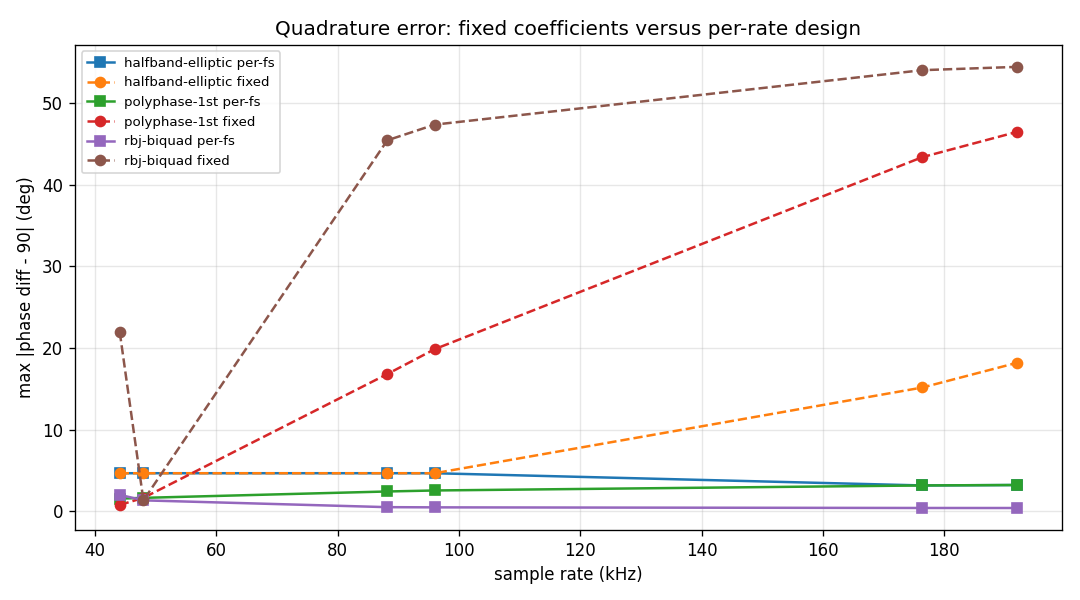
\includegraphics[width=0.85\linewidth]{fixed_vs_perfs.png}
\caption{Quadrature error versus sample rate for each topology, fixed coefficients versus per-rate design.}
\end{figure}

Per-rate coefficient redesign holds the quadrature relationship across all six
test rates for every topology.
Fixed coefficients, designed once at \SI{44.1}{\kilo\hertz} and held constant,
accumulate errors that reach \SI{54.4}{\degree} for the RBJ cascade and
\SI{46.5}{\degree} for the polyphase topology.
The elliptic half-band presents a special case: its prototype is designed in
normalised frequency, so the fixed-coefficient and per-rate columns nearly
coincide — the topology absorbs sample-rate change through frequency scaling
rather than coefficient redesign.

\subsection{Cost and Accuracy}

\begin{figure}[ht]\centering
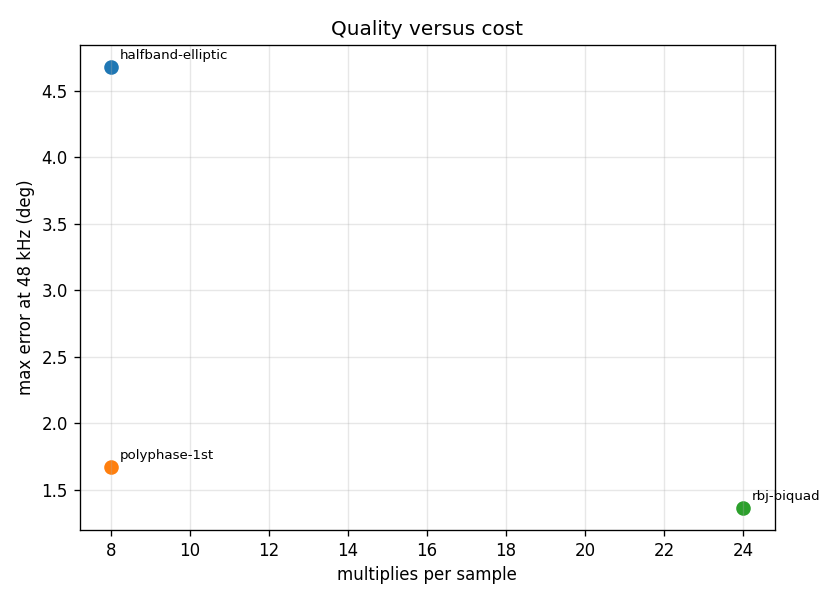
\includegraphics[width=0.7\linewidth]{pareto_cost_quality.png}
\caption{Phase accuracy at 48~kHz versus multiplies per sample.}
\end{figure}

Table~\ref{tab:results} records the three scalar figures for each topology.
The RBJ cascade achieves the lowest per-rate error at \SI{48}{\kilo\hertz}
(\SI{1.36}{\degree}) and improves to \SI{0.43}{\degree} at
\SI{192}{\kilo\hertz}, at a cost of 24 multiplies per sample.
The first-order polyphase \cite{Niemitalo2003} achieves \SI{1.67}{\degree} at
\SI{48}{\kilo\hertz} at one third of the cost (8 multiplies per sample),
making it the most accurate topology per multiply.
The elliptic half-band delivers the highest worst-case error in its design band
among the three (\SI{18.2}{\degree} in fixed mode, \SI{4.68}{\degree} per-rate
at \SI{48}{\kilo\hertz}) for the same cost of 8 multiplies.

\begin{table}[ht]
\centering
\caption{Per-topology measurements. Errors are maximum phase deviation from
\SI{90}{\degree} across the evaluation band.}
\label{tab:results}
\begin{tabular}{@{}lccc@{}}
\toprule
Topology & Cost (mult/sample) & Per-rate error at 48~kHz & Worst fixed-mode error \\
\midrule
RBJ biquad cascade           & 24 & \SI{1.36}{\degree} & \SI{54.4}{\degree} \\
Polyphase first-order        &  8 & \SI{1.67}{\degree} & \SI{46.5}{\degree} \\
Elliptic half-band           &  8 & \SI{4.68}{\degree} & \SI{18.2}{\degree} \\
\bottomrule
\end{tabular}
\end{table}

\subsection{Error Versus Filter Order}

\begin{figure}[ht]\centering
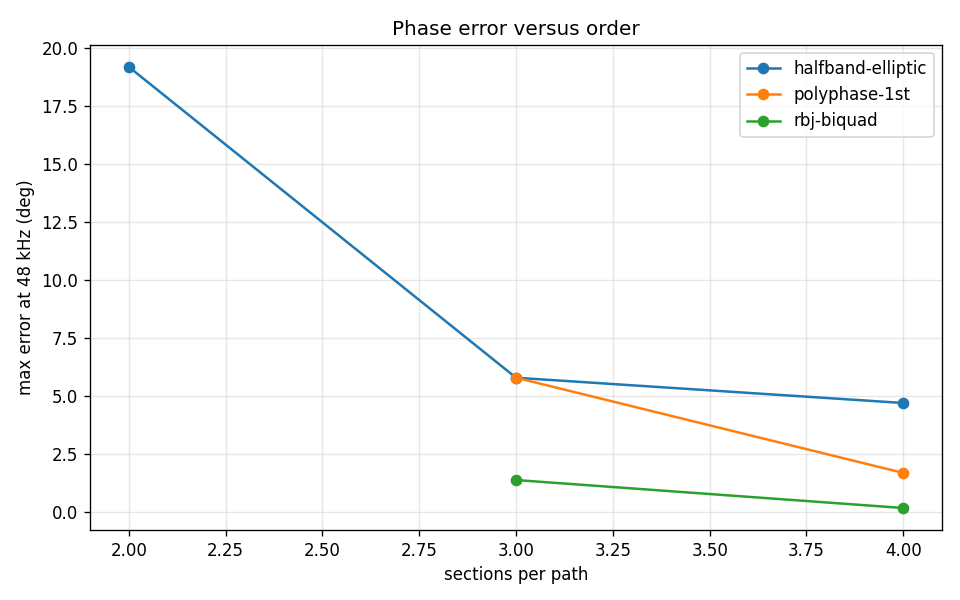
\includegraphics[width=0.8\linewidth]{error_vs_order.png}
\caption{Phase error versus the number of sections per path.}
\end{figure}

All three topologies reduce phase error monotonically as the number of
all-pass sections per path increases.
The RBJ cascade benefits most from additional sections, reaching sub-degree
accuracy at the order used in this study.
The polyphase topology converges quickly: its accuracy at 8 multiplies is
already competitive with the RBJ cascade at 24 multiplies on a per-multiply
basis.

\subsection{Differential Group Delay}

\begin{figure}[ht]\centering
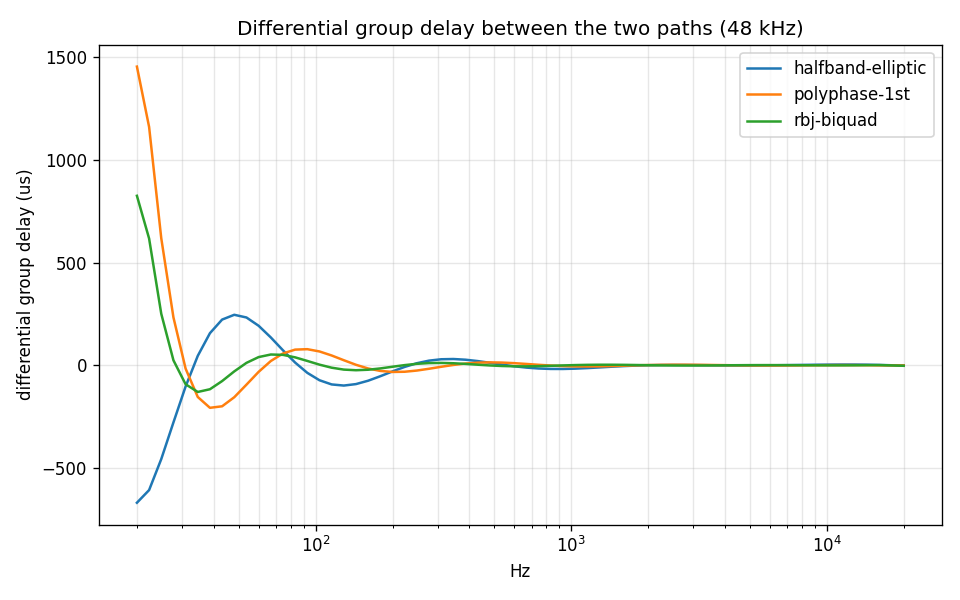
\includegraphics[width=0.8\linewidth]{group_delay.png}
\caption{Differential group delay between the two paths across frequency at 48~kHz.}
\end{figure}

The differential group delay remains small and spectrally smooth for all three
topologies at \SI{48}{\kilo\hertz}.
A near-flat differential group delay preserves transient timing relationships
between the in-phase and quadrature outputs, supporting stable spatial imaging
on percussive and speech material.

%% ─── §5 Discussion and Recommendation ───────────────────────────────────────
\section{Discussion and Recommendation}

\subsection{Sample Rate Is the Decisive Variable}

The most consistent finding across all three topologies is that the choice of
realisation mode — fixed coefficients or per-rate redesign — dominates the
accuracy outcome.
Fixed-coefficient operation produces worst-case errors above \SI{45}{\degree}
for both the RBJ and polyphase topologies, which renders them unsuitable for a
precision quadrature processor at rates other than the design rate.
Per-rate redesign, implemented as a minimax optimisation \cite{Lang1998Allpass}
that runs at host-reported sample-rate changes, reduces the worst-case error
to sub-degree range for the RBJ topology and to the 1.6–3.2-degree range for
the polyphase topology.
The elliptic half-band absorbs sample-rate variation through its normalised
frequency prototype \cite{HarrisBerdahlAbel2010,SchusslerSteffen1998}, but
delivers lower absolute accuracy at the order tested here.

\subsection{Cost–Accuracy Trade-Off}

The Pareto frontier in Figure~2 has two clear operating points.
The first-order polyphase network \cite{Niemitalo2003} sits at the
efficiency vertex: 8 multiplies per sample yield \SI{1.67}{\degree} at
\SI{48}{\kilo\hertz} and \SI{1.57}{\degree} at \SI{44.1}{\kilo\hertz}, the
best accuracy-per-multiply of the three topologies.
The RBJ biquad cascade occupies the accuracy vertex: 24 multiplies per sample
yield \SI{1.36}{\degree} at \SI{48}{\kilo\hertz} and improve to
\SI{0.43}{\degree} at \SI{192}{\kilo\hertz}, the best absolute accuracy.
The elliptic half-band shares the polyphase cost but sits below both
competitors in absolute accuracy at this order, which makes it the preferred
choice in fixed-point or very-low-MIPS contexts where its structural
regularity carries implementation advantages.

\subsection{Recommendation}

For the \texttt{x2uhj} standalone quadrature plugin, two configurations are
appropriate depending on the accuracy target.
The \emph{first-order polyphase with per-rate redesign} is the recommended
default: it delivers sub-2-degree accuracy across the audible band at one
third of the RBJ multiply count, leaving headroom for the surrounding UHJ
matrix and other processing.
The \emph{RBJ biquad cascade with per-rate redesign} is the choice when
sub-degree accuracy is required, for example in mastering or research
applications where the quadrature approximation must introduce no perceptible
artefact.
Both configurations share the same per-rate redesign requirement, which the
\texttt{x2uhj} plugin already implements through its sample-rate change
handler.
The near-flat differential group delay measured for all three topologies
confirms that none introduces perceptible pre-ringing or transient smearing on
encoded material, supporting their use on broadband programme.

%% ─── §6 References ───────────────────────────────────────────────────────────
\section*{References}

\bibliographystyle{IEEEtran}
\bibliography{../../doc/math/refs}
\end{document}
